\documentclass[a4paper,11pt]{article}
\usepackage{geometry}
\geometry{
 a4paper,
 total={170mm,267mm},
 left=20mm,
 top=10mm,
 }
 \usepackage[utf8]{inputenc}
% \usepackage{ibcat5ia}
% \usepackage{opencolor}
\usepackage[utf8]{inputenc}
\usepackage[toc,page]{appendix}
\usepackage{listings}
%\usepackage{pdfpages}
%\usepackage{subfig}
\usepackage{minted}
%\usepackage{subcaption} 
%\usepackage{soul}
%\usepackage{float}
%\usepackage{graphicx}
\usepackage{pgfplots}
\usepackage[english]{babel}
\usepackage{svg}
\usepackage{kpfonts}
\usepackage{multicol}
\usepackage{blindtext}
\setlength{\columnsep}{4em}


\begin{document}
\author[1]{Sergio Gómez}
\author[]{Apuntes ER}
\begin{multicols*}{2}
	\section{Soroll térmic}
	Depèn de la temperatura T del conductor.
	Temperatura de referencia:
	$$T=ºC+273\rightarrow T_0=17ºC=290K$$
	Densidad espectral de potencia:\\
	$S_n=kT$ amb $k=1.38\cdot10^{-23}\frac{W}{Hz\cdot K}$\\
	Es un soroll blanc ja que no depen de la frequencia.\\
	Potencia de soroll $P_n=kTB$ en W\\
	$$P_{dBm}=P_{dBW}+30\ dB$$
	 
	\section{Soroll en quadripols}
	Un quadripol no ideal es pot modelar com si fos ideal incrementant la temperatura de la señal de entrada
	
	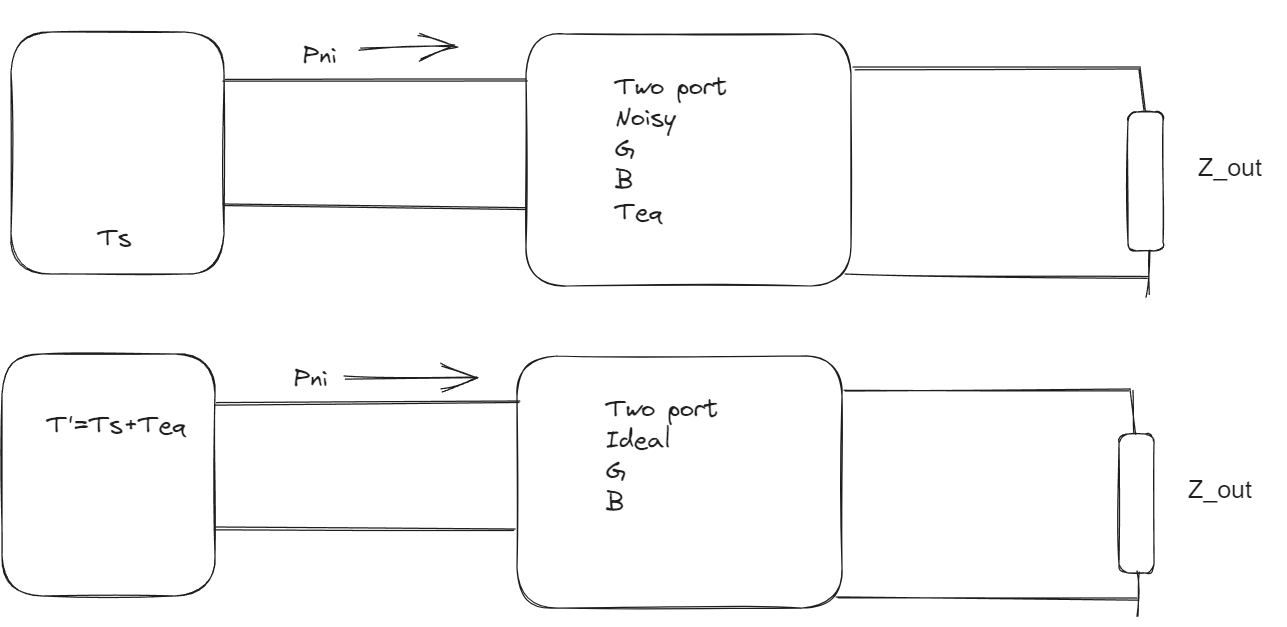
\includegraphics[width=1\linewidth]{Screenshot 2023-10-21 123320.png}
	$$P_{no}=P_{ni}G+P_{no}'=k(T_s+T_e)BG$$
	$$T_e=\frac{P_{no}}{kBG}$$
	\subsection{Relació señal soroll}
	$(S/N)_i=\frac{P_{si}}{P_{ni}}$ per a la entrada i $(S/N)_o=\frac{P_{so}}{P_{no}}$
	$$(S/N)_o=\frac{(S/N)_i}{1+\frac{T_{eq}}{T_{in}}}$$
	\subsection{Factor de soroll}
	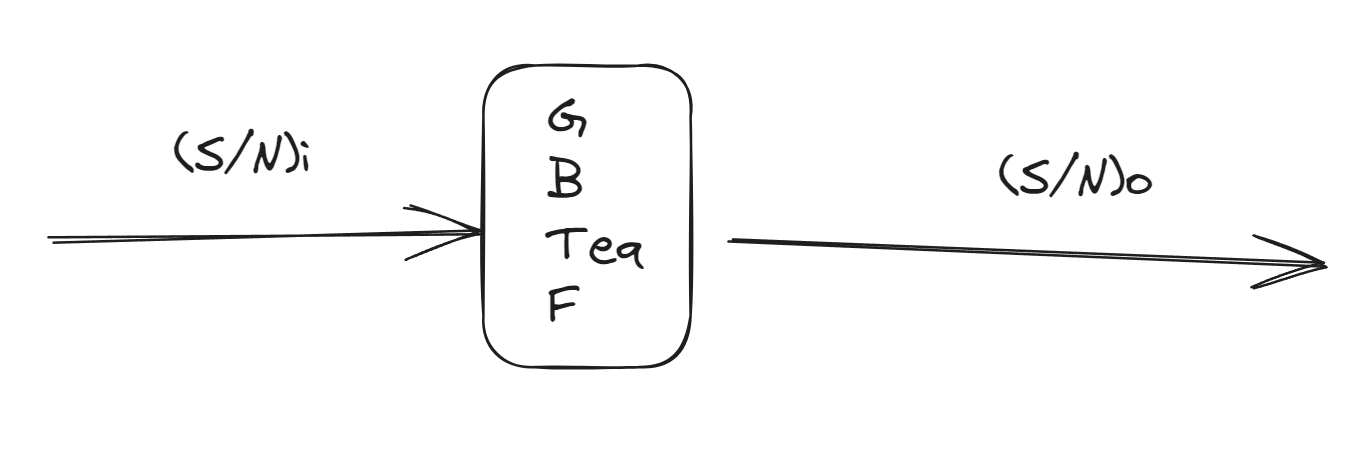
\includegraphics[width=1\linewidth]{quaddiagram.png}
		
	$$F=\frac{\text{Potencia quad sorollos}}{\text{Potecia si el quad fos ideal}}$$
	$F\leq1$;$F=1+\frac{T_{eq}}{T_0}\Leftrightarrow T_e=(F-1)T_0$\\
	Noise figure: $NF=10\log(F)[dB]$
	\subsection{Atenuador passiu}
	No amplifica, només té perdues
	$$P_n=kT_{phy}B$$
	$$G=\frac{1}{L}\rightarrow 10\log L=-10\log G$$
	$$T_{eq}=LT_{phy}-T_{in}$$
	$$F= 1+\frac{T_{eq}}{T_0}(L-1)$$
	\subsection{Adaptacio de impedancies}
	$$P_{no}=k(T_{phy}+T_{eq})B\frac{1}{L} $$
	\section{Formula de Friis}
	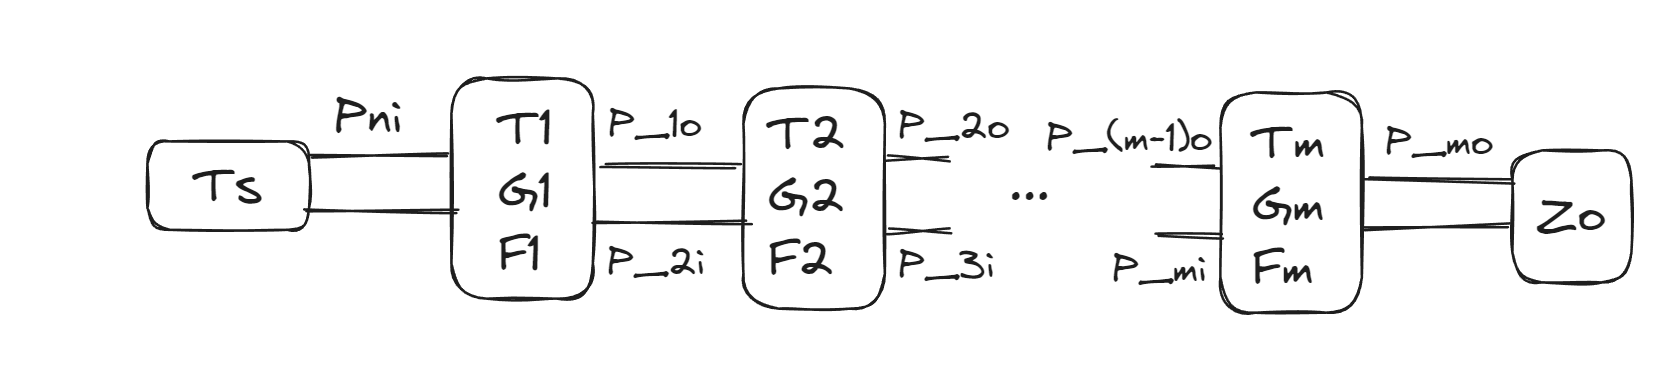
\includegraphics[width=1\linewidth]{quadcascada.png}
	$$T_{eq}=T_1+\frac{T_2}{G1}+\frac{T_3}{G_1 G_2}+\dots+\frac{T_m}{G_1 G_2\dots G_{m-1}}$$
	$$F=F_1+\frac{F_2-1}{G1}+\frac{F_3-1}{G_1 G_2}+\dots`\frac{F_m-1}{G_1 G_2\dots G_{m-1}}$$
	$$(S/N)_o=\frac{(S/N)_i}{1+\frac{T_{eq}}{T_in}}=\frac{(S/N)_i}{1+\frac{T_0}{T_in}(F-1)}$$
		
	\section{Receptor}
	\subsection{Sensibilitat}
	Per a $T_{in}=T_0$
	$$S_{in_{min}}=N_{in}F(S/N)_{out}=kT_0GF(S/N)_{o}$$
	\subsection{Mínim senyal detectable(MDS)}
	$$MDS_{in}=N_{in}=F(S/N)_{out}=kT_0BF$$
	\subsection{Marge dinàmic(DR)}
	$$DR[dB]=S_{in}|_{max}[dBm]-MDS_{in}[dBm]$$
	 
	\section{Distorció harmonica i intermodulació}
	\subsection{Intermodulation ratio(IMR)}
	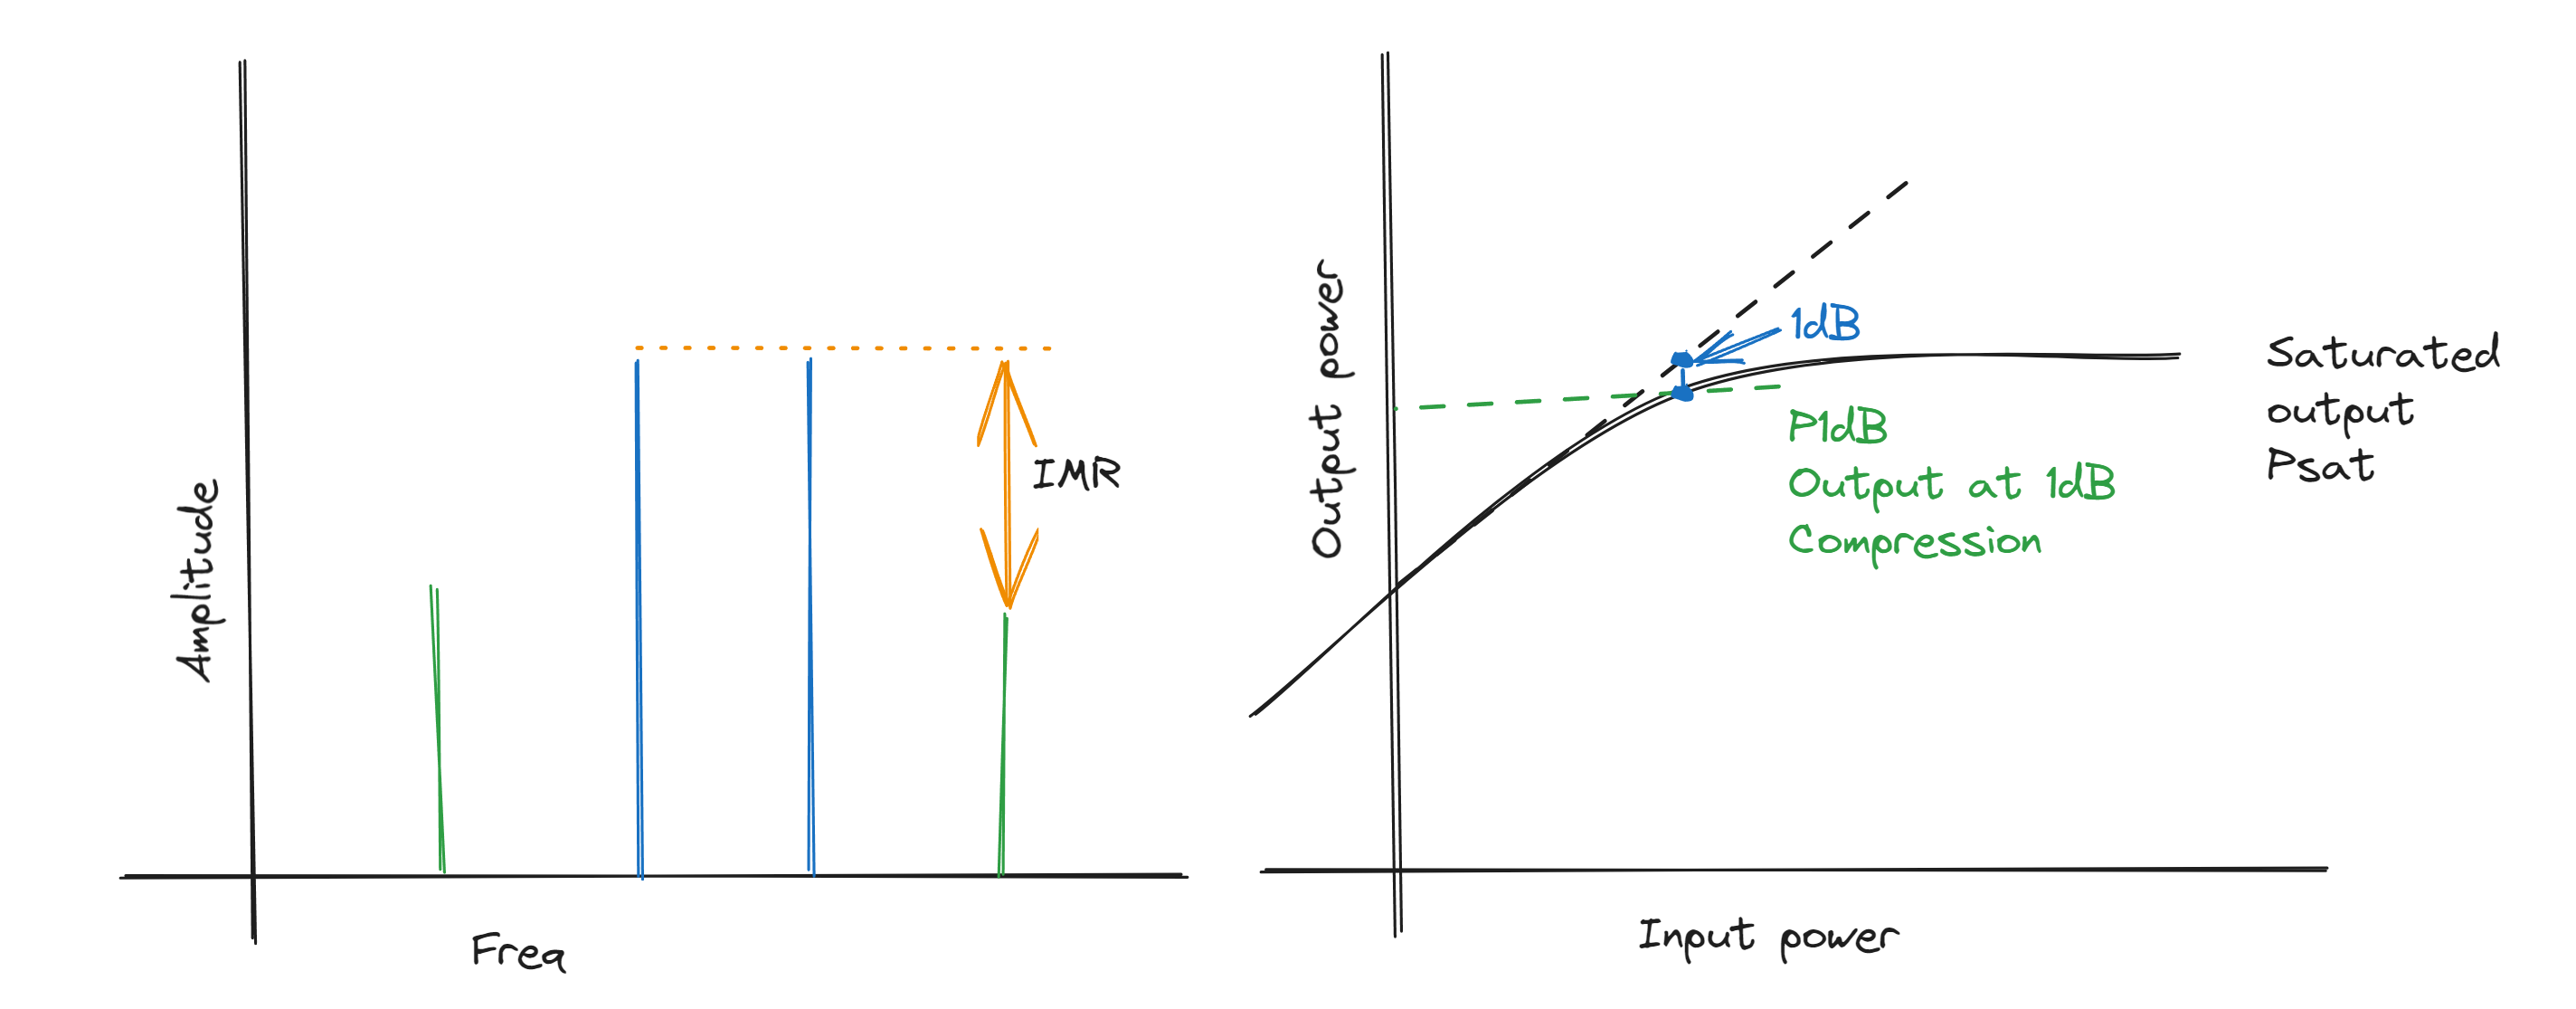
\includegraphics[width=1\linewidth]{IMRcompresion.png}
	
	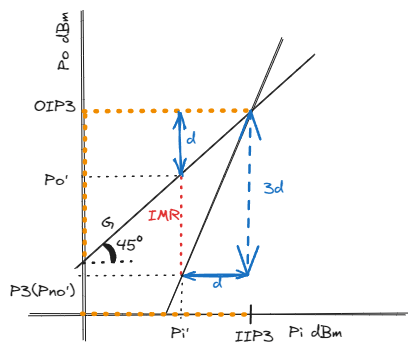
\includegraphics[width=1\linewidth]{OIPIIP3.png}
	$$IMR(Pi)=P_o[dBm]-P_3[dBm] [dB]$$
	$$IIP_3=P_i+\frac{IMR}{2} [dBm]$$
	$$OIP_3=P_0+\frac{IMR}{2} [dBm]$$
	$$IMD=P_o-IMR$$
	\subsection{Spureos free dynamic range(SFDR)}
	$$MDS_{in}=P_{ni}'=k(T_s+T_e)B [W]$$
	$$MDS_{out}=P_{no}=P_{ni}'+20\log a_1 [dBm]=k(T_s+T_e)Ba_1^2$$
	$$SFDR=\frac{2}{3}(IIP_3-MDS_{in})=\frac{2}{3}(OIP_3-MDS_{out})=P_i-MDS_{in} $$
	\section{Radioenllaços}
	$$FSL=(\frac{\lambda}{4\pi d})^2$$
	$$P_r=PIRE\cdot G_R\cdot FSL=P_t\cdot G_t\cdot G_R\cdot FSL$$
\end{multicols*}

\end{document}